\chapter{Scattering Model}\label{chapter:scattering_model}
A system of three identical bosons with $J=0$ and masses $m = m( \prescript{87}{}{\mathrm{Rb}})$ has been considered in this work. We have assumed that the interactions $V(\rho,\theta,\psi)$ can be written as a sum of pairwise two-body potentials   

\begin{equation}\label{eq:potential_sum}
V(\rho,\theta,\psi) = v(r_{12}) + v(r_{23}) + v(r_{31}).
\end{equation} 

Since a general feature of the Efimov effect is that it is insensitive to the details of the short-ranged interatomic interactions and that it, to a good approximation, only depends on the scattering length and the interaction range it allows for the use of model potentials, where the scattering length and the number of two-body bound states can be controlled. The two-body potential used here is  

\begin{equation}\label{eq:two_b_potential}
v(r) = -d\cosh^{-2}{(r/r_0)},
\end{equation}
where $d$ controls the depth and $r_0$ the range of the potential. This potential is particularly useful since the eigenfunctions and energies are known analytically \cite{Landau1965Quantum}. The scattering length can be calculated at different $d$ numerically as described in \cref{sec:zero_energy_scat}, or can be expressed analytically as a function of $d$ through 

\begin{equation}
a = \lim_{k \to 0} \frac{1}{ik} \frac{S(k)-1}{S(k)+1}
\end{equation}
in which $S(k)$ is the diagonal S-matrix element given by

\begin{equation}
S(k) = 2^{\varepsilon} \frac{\,_2F_1(-s, s+1, 1-\varepsilon;\frac{1}{2})}{\,_2F_1(\varepsilon-s, \varepsilon + s+1, 1+\varepsilon;\frac{1}{2})},
\end{equation}
where $\,_2F_1$ is the hypergeometrical function, $\varepsilon = ikr_0$, $k = \sqrt{mE_{2\mathrm{b}}}$, $s = \frac{1}{2}(-1 + \sqrt{1-4 m d r_0^2})$. The two-body $s$-wave eigenenergies are given by

\begin{equation}\label{eq:exact_2b}
E_{2\mathrm{b}} = -\frac{\Big(-(1+2n)+\sqrt{1-4mdr_0^2}\Big)^2}{4mr_0^2}.
\end{equation}

The binding energy for the shallow dimer for $a>0$ is universal and can be well approximated by equation \eqref{shallowdimer} if the scattering length is sufficiently large.

The scattering length is plotted as a function of the potential depth in \cref{fig:res_1} using the range $r_0=55 $ a.u. and the mass of $ \prescript{87}{}{\mathrm{Rb}}$, which is precisely the same results as in \cite{Blume2002}. By changing the depth $d$, the potential can be tuned to support a different number of two-body bound $s$-wave states. The formation of a two-body bound state can be recognized by the scattering length going through a pole. Three such poles can be seen in \cref{fig:res_1}, labelled $\mathrm{I},\mathrm{II}$ and $\mathrm{III}$. At each pole a new bound state is formed. The first weakly bound dimer is formed as $a$ passes through $\mathrm{I}$ from the left. Then, as $a$ approaches $\mathrm{II}$ the first bound state becomes deeply bound and a second bound state is formed as $a$ goes through $\mathrm{II}$ and again becomes positive. A third bound state is formed in the same manner as $a$ passes over $\mathrm{III}$ to the positive side.

\begin{figure*}[b!]
	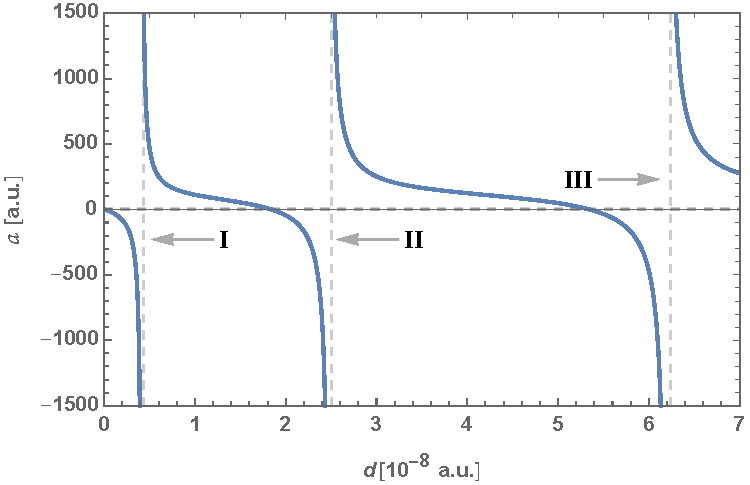
\includegraphics[width=\linewidth]{scattering_new.pdf}
	\caption{The two-body scattering length as a function of the potential depth $d$. Three poles can be recognized in the figure, labelled $\mathrm{I},\mathrm{II}$ and $\mathrm{III}$. For values of $d$ that lie between the poles $\mathrm{I}$ and $\mathrm{II}$, the potential is deep enough to support a single $s$-wave bound state.}
	\label{fig:res_1}
\end{figure*}

The two-body potential surfaces $V(\rho,\theta,\phi)$ for two different hyperradii $\rho$ are shown in \Cref{fig:surfaces}. The potential surface can be seen to change more rapidly near the hyperangular configurations $(\theta,\phi)=(\pi/2,\phi)$ for larger $\rho$. 

\begin{figure}[htbp!]
	\centering
	\subcaptionbox{The potential surface for $\rho=r_0$.}{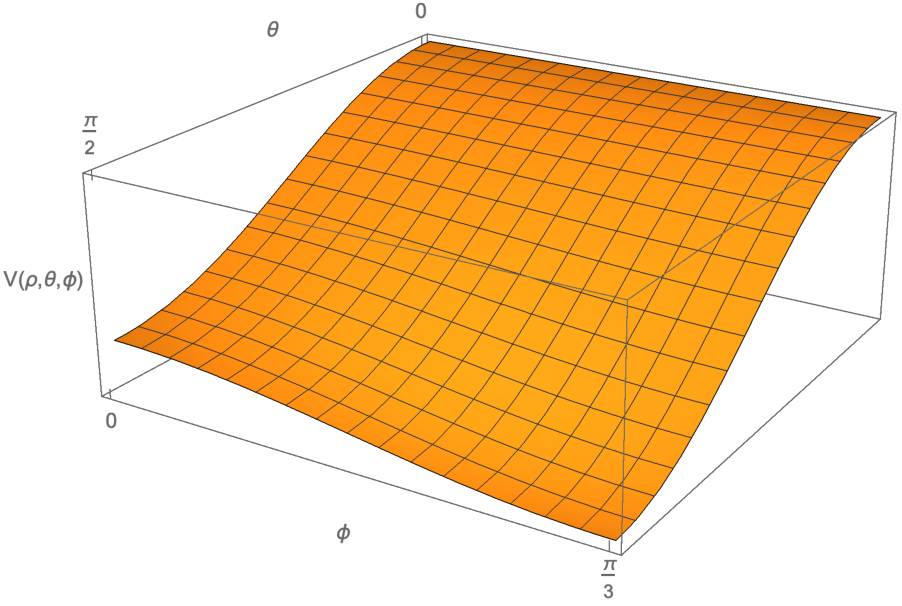
\includegraphics[width=0.5\textwidth]{surface_small.pdf}}%
	\hfill % <-- Seperation
	\subcaptionbox{The potential surface for $\rho=3r_0$.}{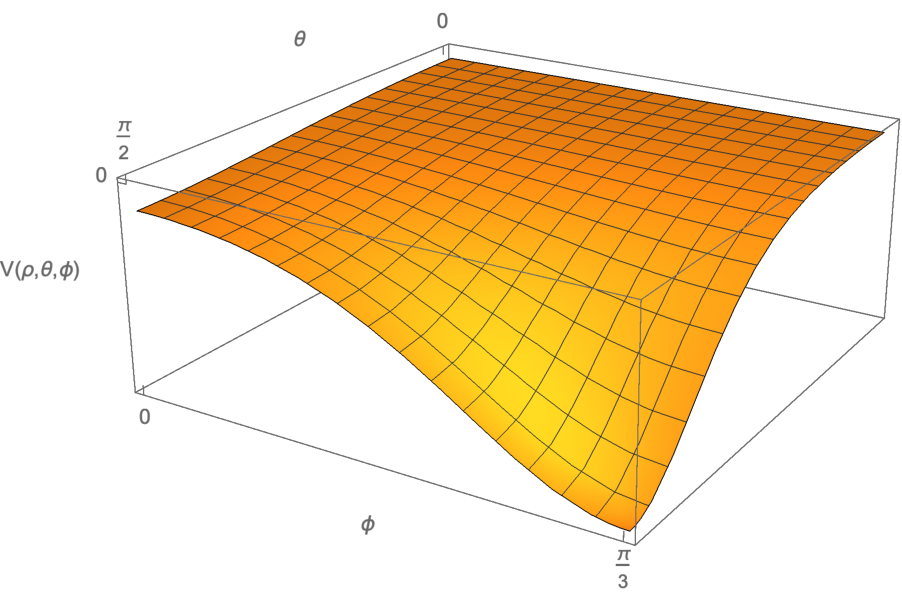
\includegraphics[width=0.5\textwidth]{surface_large.pdf}}%
	\caption{Illustration of the two-body potential surfaces at two different hyperradii $\rho$. The potential surface change more rapidly at the hyperangular configuration $(\theta,\phi)=(\pi/2,\phi)$ for larger $\rho$.}\label{fig:surfaces}
\end{figure}
